\documentclass[12pt]{article}
\usepackage[utf8]{inputenc}
\usepackage[spanish]{babel}
\usepackage{graphicx}
\usepackage{float} 
\usepackage{url}
\usepackage{listingsutf8}
\usepackage{color}
%\usepackage{listingsutf8}
%\usepackage{amsmath,amssymb}
\usepackage[nottoc,notlot,notlof]{tocbibind} % Hace que se agregen las referencias al indice

\definecolor{codegreen}{rgb}{0,0.6,0}
\definecolor{codegray}{rgb}{0.5,0.5,0.5}
\definecolor{codepurple}{rgb}{0.58,0,0.82}
\definecolor{backcolour}{rgb}{0.95,0.95,0.92}

\lstdefinestyle{mystyle}{
	backgroundcolor=\color{backcolour},   
	commentstyle=\color{codegreen},
	keywordstyle=\color{magenta},
	numberstyle=\tiny\color{codegray},
	stringstyle=\color{codepurple},
	basicstyle=\footnotesize,
	breakatwhitespace=false,         
	breaklines=true,                 
	captionpos=b,                    
	keepspaces=true,                 
	numbers=left,                    
	numbersep=5pt,                  
	showspaces=false,                
	showstringspaces=false,
	showtabs=false,                  
	tabsize=2
}

\lstset{
	style=mystyle,
	inputencoding=utf8/latin1
}

% Title Page
\title{Simulación Juego de la Vida - Gráfica de promedio de unos y densidad}
\author{Alumno: Monroy Martos Elioth \\ Profesor: Genaro Juárez Martínez \\ Materia: Computing Selected Topics \\ Grupo: 3CM8}


\begin{document}
\maketitle
\newpage
\tableofcontents
% \newpage
% \section{Introducción}
	El juego de la vida fue desarrollado por John Horton Conway, quien fuera un matemático estadounidense que trabajaba en la Universidad de Cambridge. Él desarrollo un ``juego'' al cual llamaba vida, debido a su parecido con la forma en que las sociedades de organismos vivos se levantan y caen.\cite{web}

	Este juego se considera como un simulador, ya que se asemeja a la vida real. Originalmente, se planteó como un juego de mesa, pero con el pasar de los años fue usado en otras ramas (como la computación) debido a las posibilidades que este juego brinda.

	La idea básica del juego, es iniciar con una configuración simple de organismos vivientes, cada uno asignado a una celda dentro de un tablero (el cual se considera un plano infinito), para así observar como está cambia según se aplican las leyes genéticas de Conway, las cuales determinan el nacimiento, muerte o supervivencia de cada organismo. Estás reglas son tres:
	\begin{enumerate}
		\item Supervivencia: Cada organismo con dos o tres vecinos vivos sobrevivirá a la siguiente generación.
		\item Muerte: Cada organismo con cuatro o más vecinos muere por sobrepoblación, así mismo cada organismo con solo un vecino o ninguno morirá por aislamiento.
		\item Nacimiento: En cada celda vacía que este rodeada por exactamente tres vecinos, nacerá un organismo. \cite{web}
	\end{enumerate}

	Es importante señalar que cada muerte, nacimiento o supervivencia debe ser simultaneo durante cada salto de generación.
	Para realizar la evaluación de cada una de las celdas, estás son divididas a su vez en grupos de 9 celdas, la célula que se evaluará constituye el centro del ahora cuadrado. Dentro de este cuadrado, son aplicadas las reglas ya descritas anteriormente.

	El programa que ha sido desarrollado para está actividad, simula este juego. Son dados como parámetros el total de la población y la probabilidad de que existan organismos vivos en la misma. Y con base a esto se realizada la simulación del juego de la vida aplicando las reglas de Conway. Además se gráfica el histórico de la cantidad de organismos vivos que han existido durante cada una de las generaciones.
\newpage
\section{Desarrollo}
	Para la elaboración del programa, se realizó el siguiente diagrama que modela los estados y las transiciones que tiene la máquina.

	\begin{figure}[H]
		\begin{center}
			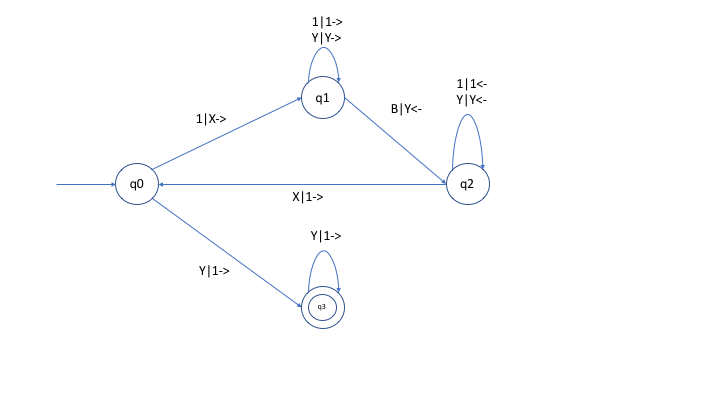
\includegraphics[scale=.4]{img/maquina.png}
			\caption{Estados y transiciones usados}
			\label{fig:maquina}
		\end{center}
	\end{figure}

	Posteriormente, para el modelado de la máquina de Turing se realizó la siguiente implementación en Python 3.7, la cual es una clase que sirve para trabajar con la misma:

	maquina.py
	\lstinputlisting[language=Python]{../maquina.py}

	Por si sola está máquina no tiene funcionalidad, por lo cual fue necesario el uso de la misma en otro archivo, el cual se encarga de manejar todo el funcionamiento del programa, como recibir la entrada (cadena de unos), y utilizar tkinter para realizar la animación de la máquina de Turing.
	\lstinputlisting[language=Python]{../main.py}
% \newpage
% \section{Resultados}
	Para comprobar la funcionalidad del programa, primero probaré ingresando un AFD y posteriormente un AFND
	\paragraph{AFD}
	El AFD que creará nuestra clase AFD es el siguiente:
	\begin{figure}[H]
		\begin{center}
			\includegraphics[width=10cm, height=4cm]{img/afd_auto.png}
			\caption{AFD de Prueba}
			\label{fig:tablas}
		\end{center}
	\end{figure}
	Este autómata solo acepta la cadena '01'. Cualquier otra cadena sería invalida.\\
	El archivo de entrada para la creación de este autómata, luce de la siguiente manera:
	\begin{figure}[H]
		\begin{center}
			\includegraphics[width=6cm, height=4cm]{img/afd_entrada.png}
			\caption{Archivo de entrada para el AFD}
			\label{fig:tablas}
		\end{center}
	\end{figure}
	Al ejecutar el programa e ingresar el archivo, y posteriormente las cadenas, obtenemos las salidas esperadas.
	\begin{figure}[H]
		\begin{center}
			\includegraphics[width=15cm, height=10cm]{img/afd_salida.png}
			\caption{Ejecución y pruebas del AFD}
			\label{fig:tablas}
		\end{center}
	\end{figure}
	\newpage
	\paragraph{AFND}
	El AFND que creará nuestra clase AFND es el siguiente:
	\begin{figure}[H]
		\begin{center}
			\includegraphics[width=10cm, height=4cm]{img/afnd_auto.png}
			\caption{AFND de Prueba}
			\label{fig:tablas}
		\end{center}
	\end{figure}
	Cabe señalar, que las transiciones epsilon son representadas por el símbolo '\textdollar'.\\
	Este autómata acepta la cadena '001x' por ejemplo, en general acepta cualquier cadena la cual empiece con cualquier cantidad de '0' o '1' pero que siempre al final lleve la siguiente combinación '1x'. Cualquier otra cadena sería invalida, por ejemplo, cadena '00x1'.\\
	El archivo de entrada para la creación de este autómata, luce de la siguiente manera:
	\begin{figure}[H]
		\begin{center}
			\includegraphics[width=12cm, height=5cm]{img/afnd_entrada.png}
			\caption{Archivo de entrada para el AFND}
			\label{fig:tablas}
		\end{center}
	\end{figure}
	\newpage
	Al ejecutar el programa e ingresar el archivo, y posteriormente las cadenas, obtenemos las salidas esperadas.
	\begin{figure}[H]
		\begin{center}
			\includegraphics[width=15cm, height=10cm]{img/afnd_salida.png}
			\caption{Ejecución y pruebas del AFND}
			\label{fig:tablas}
		\end{center}
	\end{figure}
% \newpage
% \section{Conclusiones}
	El uso de autómatas finitos deterministas y no deterministas nos permite validar que el orden en cadenas de entrada sea correcto.
	Esto tiene diversas aplicaciones, desde muy sencillas (como validar el formato de un CURP) hasta aplicaciones más complejas como realizar parte del análisis léxico de un lenguaje de entrada en un compilador.\\Los cuales nos ayudan a saber si una entrada pertenece a nuestro lenguaje o no, siendo de gran utilidad al momento de validar cadenas apartir de una expresión regular.

% \bibliographystyle{ieeetr}
% \bibliography{referencias}

%\cite{macy}

\end{document}
